%%% LaTeX Template: Article/Thesis/etc. with colored headings and special fonts
%%%
%%% Source: http://www.howtotex.com/
%%% Feel free to distribute this template, but please keep to referal to http://www.howtotex.com/ here.
%%% February 2011
%%%
%%% Modified January 2016 by CDM

%%%  Preamble
\documentclass[11pt,letterpaper]{article}
\usepackage[margin=1.0in]{geometry}
\usepackage[T1]{fontenc}
\usepackage[bitstream-charter]{mathdesign}
\usepackage[latin1]{inputenc}					
\usepackage{amsmath}						
\usepackage{xcolor}
\usepackage{cite}
\usepackage{hyphenat}
\usepackage{graphicx}
\usepackage{float}
\usepackage{subfigure}
\usepackage{sectsty}
\usepackage[compact]{titlesec} 
\usepackage[tablegrid]{vhistory}
\usepackage{pbox}
\allsectionsfont{\color{accentcolor}\scshape\selectfont}

%%% Definitions
\definecolor{accentcolor}{rgb}{0.0,0.0,0.5} 
\newcommand{\teamname}{Team IDP}
\newcommand{\productname}{Interactive Degree Planner}
\newcommand{\coursename}{CSE 4316: Senior Design I}
\newcommand{\semester}{Fall 2021}
\newcommand{\docname}{Architectural Design Specification}
\newcommand{\department}{Department of Computer Science \& Engineering}
\newcommand{\university}{The University of Texas at Arlington}
\newcommand{\authors}{Daniel Newville \\ Le Uyen Nguyen \\ Ijaz Mohamed Umar \\ Safi Ullah}

%%% Headers and footers
\usepackage{fancyhdr}
	\pagestyle{fancy}						% Enabling the custom headers/footers
\usepackage{lastpage}	
	% Header (empty)
	\lhead{}
	\chead{}
	\rhead{}
	% Footer
	\lfoot{\footnotesize \teamname \ - \semester}
	\cfoot{}
	\rfoot{\footnotesize page \thepage\ of \pageref{LastPage}}	% "Page 1 of 2"
	\renewcommand{\headrulewidth}{0.0pt}
	\renewcommand{\footrulewidth}{0.4pt}

%%% Change the abstract environment
\usepackage[runin]{abstract}			% runin option for a run-in title
%\setlength\absleftindent{30pt}			% left margin
%\setlength\absrightindent{30pt}		% right margin
\abslabeldelim{\quad}	
\setlength{\abstitleskip}{-10pt}
\renewcommand{\abstractname}{}
\renewcommand{\abstracttextfont}{\color{accentcolor} \small \slshape}	% slanted text

%%% Start of the document
\begin{document}

%%% Cover sheet
{\centering \huge \color{accentcolor} \sc \textbf{\department \\ \university} \par}
\vspace{1 in}
{\centering \huge \color{accentcolor} \sc \textbf{\docname \\ \coursename \\ \semester} \par}
\vspace{0.5 in}
\begin{figure}[h!]
	\centering
   	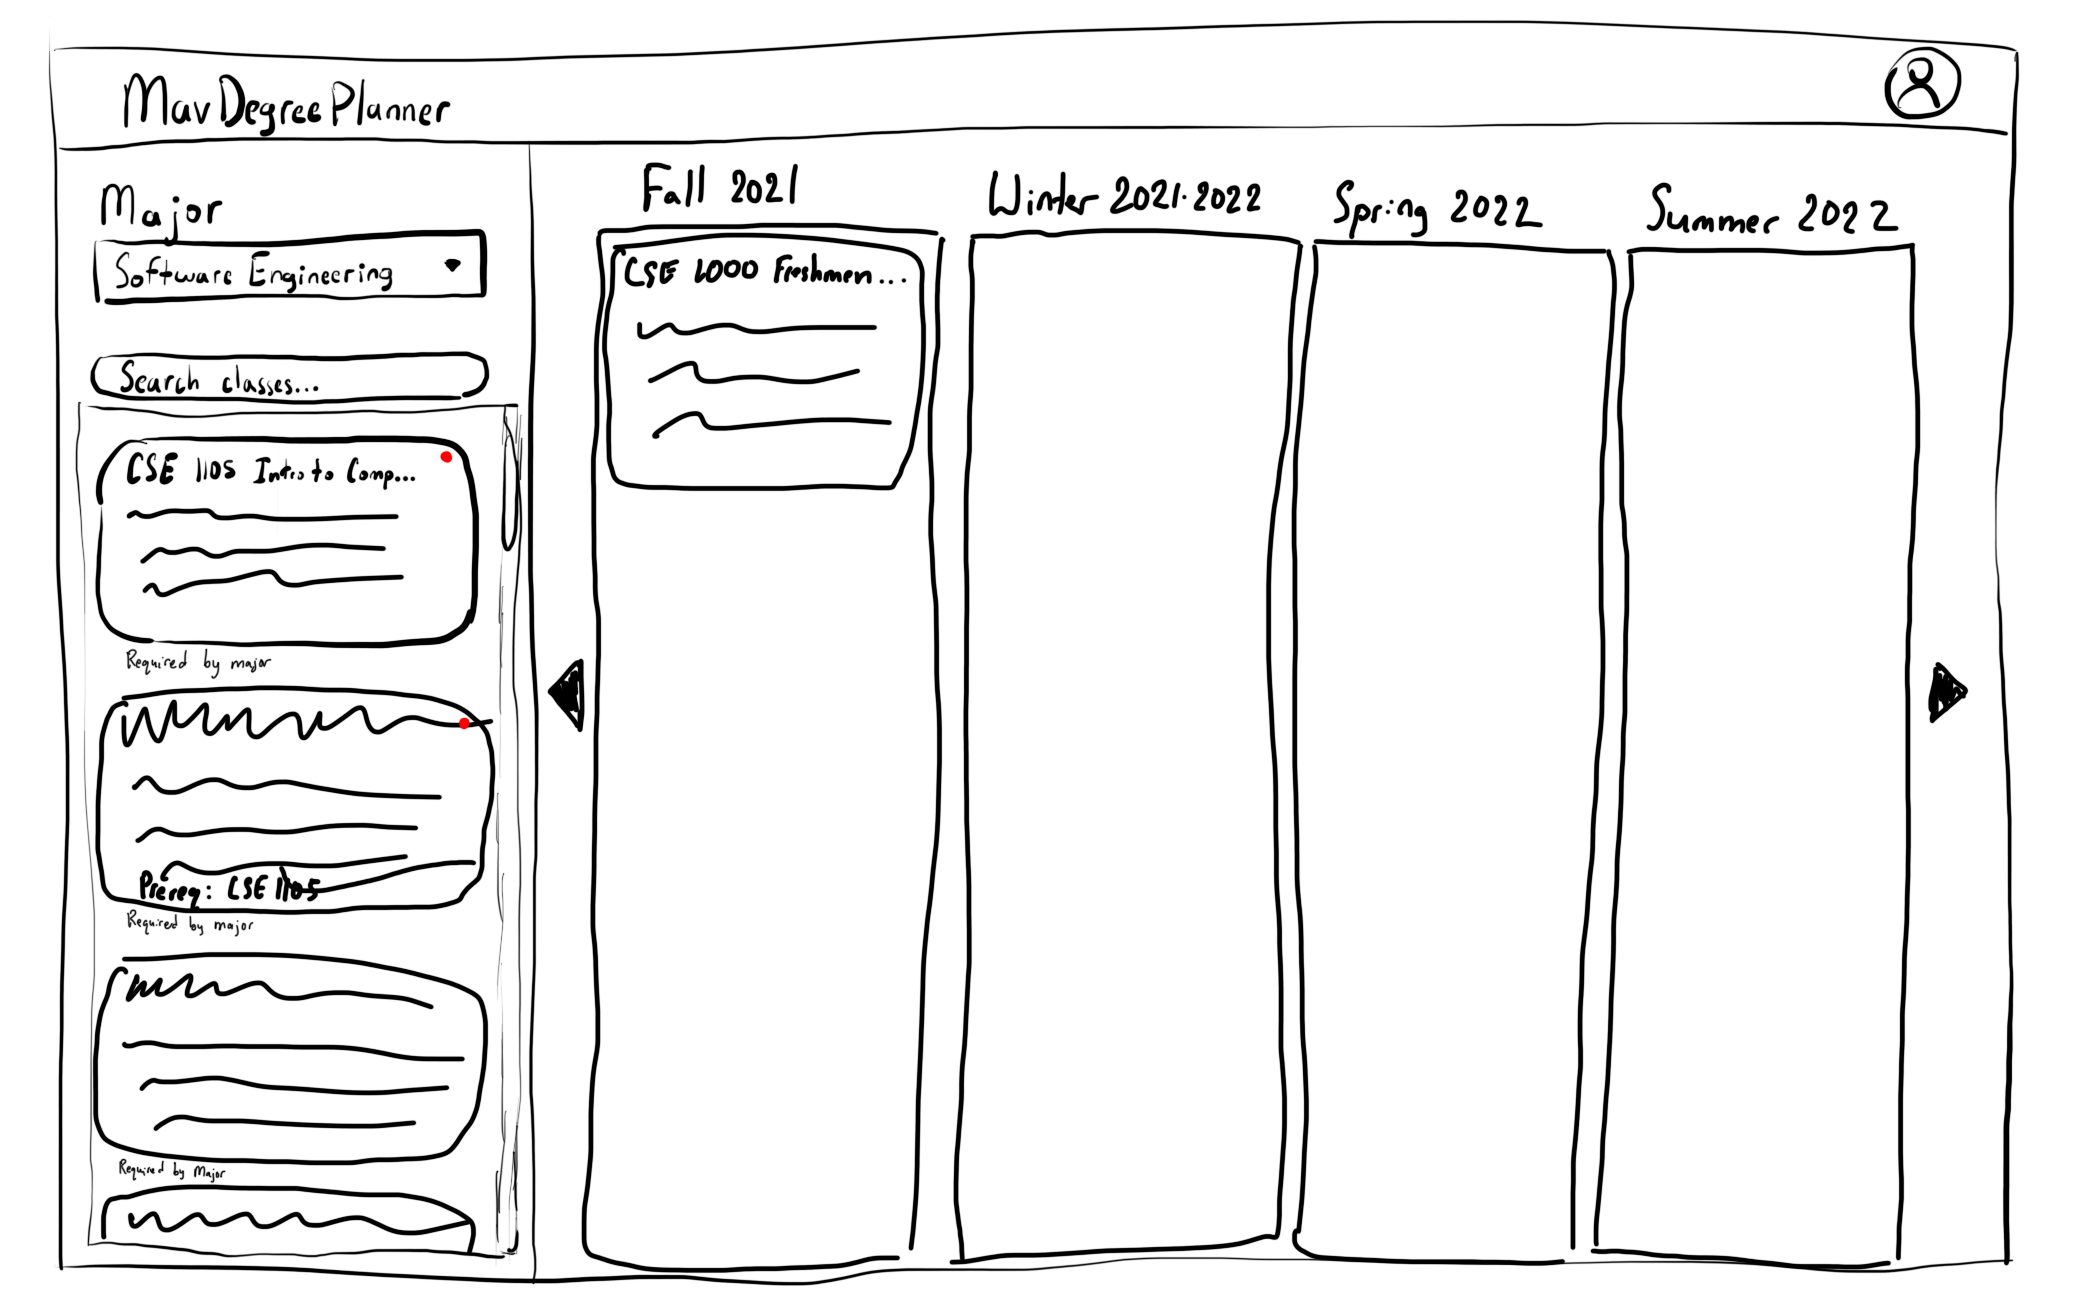
\includegraphics[width=0.60\textwidth]{images/MavDegreePlannerDiagram}
\end{figure}
\vspace{0.5 in}
{\centering \huge \color{accentcolor} \sc \textbf{\teamname \\ \productname} \par}
\vspace{0.5 in}
{\centering \large \sc \textbf{\authors} \par}
\newpage


%\vspace{1 in}
%\centerline{January 13th, 2012}
%\newpage

%%% Revision History
\begin{versionhistory}
  	\vhEntry{0.1}{12.04.2021}{DN}{document creation}
  	\vhEntry{0.2}{12.10.2021}{Group}{document completion}
  	\vhEntry{0.3}{05.07.2021}{Group}{document revision}
\end{versionhistory}
\newpage

%%% Table of contents
\setcounter{tocdepth}{2}
\tableofcontents
\newpage

%%% List of figures and tables (optional)
\listoffigures
\listoftables
\newpage

%%% Document sections
\section{Introduction}
Your introduction should describe your product concept in sufficient detail that the architectural design will be easy to follow. The introduction may include information used in the first sections of your SRS for this purpose. At a minimum, ensure that the product concept, scope and key requirements are described.
\newpage
\section{System Overview}
The website will consist of a side panel with a list of classes and the main
    screen with columns for each semester. It will also have a section for user accounts.

The user can sign up for an account to access their plan anywhere. The system
    will support signin, signout, and forgot password. The system will collect email and
    password for signup and signin.

The side panel lists all classes available to a student. At the top of the side panel,
    the user can choose their major to check their classes against for pre/coreqs.
    Classes required by a student's major will be shown at the top, other classes
    will be at the bottom. It will show required classes that have satisfied
    the prereq and coreq requirements at the top of the list required classes section.
    The list of classes is also searchable. The major and chosen classes are saved
    to the user's account so they can access it later.

The main screen consists of a horizontably scrollable list of semesters. Each
    semester has a list of classes that the user has chosen. The first semester
    shown on the screen is the current one.

Each class can be dragged from the side panel to a semester's list of classes.
    The class will have an error above it if the user has not taken a prereq/coreq class
    in a previous semester, or if the user has not chosen a coreq in the same
    semester.
    
\begin{figure}[h!]
    \centering
    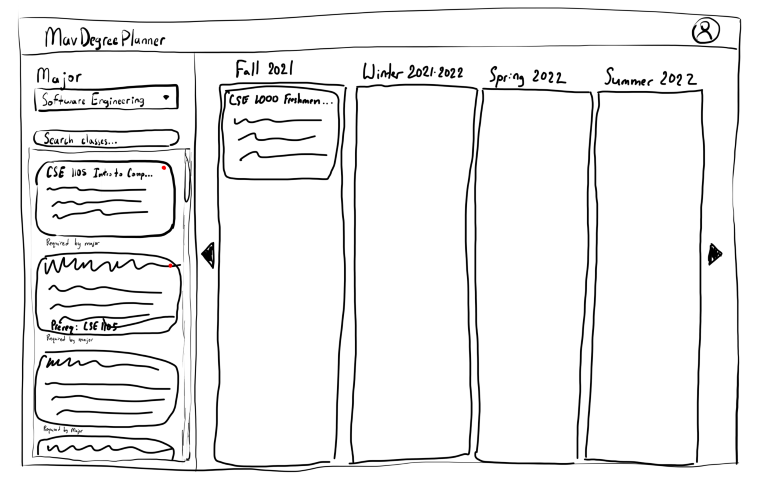
\includegraphics[width=0.5\textwidth]{images/MavDegreePlannerDiagram-Small} % Image
    \caption{Diagram of Major System Components} % Caption
\end{figure}
\newpage
\section{Subsystem Definitions \& Data Flow}
This section breaks down your layer abstraction to another level of detail. Here you grapically represent the logical subsytems that compose each layer and show the interactions/interfaces between those subsystems. A subsystem can be thought of as a programming unit that implements one of the major functions of the layer. It, therefore, has data elements that serve as source/sinks for other subsystems. The logical data elements that flow between subsystems need to be explicitly defined at this point, beginning with a data flow-like diagram based on the block diagram.

%%%%%%%%%%%%%%%%%%%%%%%%%%%%%%%%%%%%%%%%%%%%%%%%%%%%%%%%%%
%  BE SURE TO UPDATE THE IMAGE CAPTION
\begin{figure}[h!]
	\centering
 	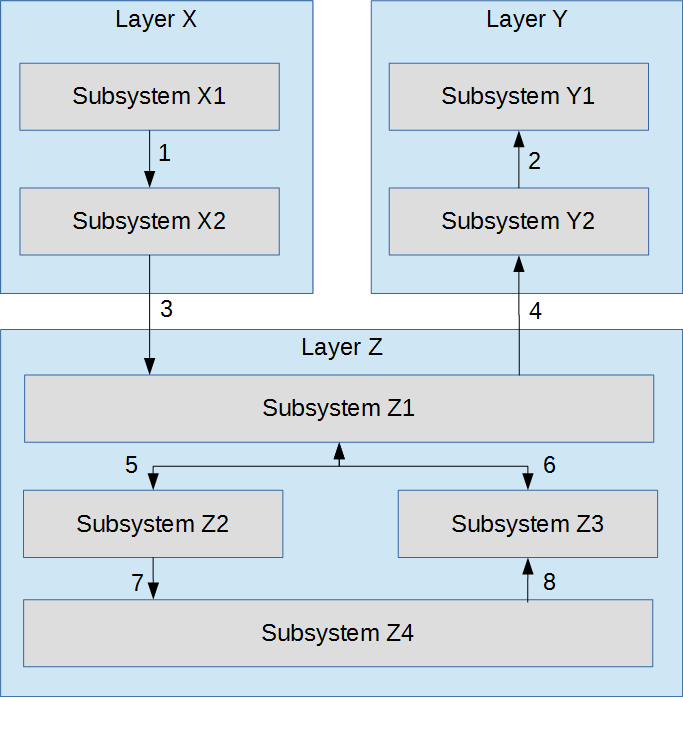
\includegraphics[width=\textwidth]{images/data_flow} % Image
 \caption{A simple data flow diagram} % Caption
\end{figure}

\newpage
\section{Degree Planner UI Layer}
The Degree Planner UI layer consists of Web application, Course catalog, Semester catalog, and Export subsystem. The main functionality of this layer is to provide the user interface, where the user is able to prepare his/her degree plan and view the related information. Among the above-mentioned subsystems, the Web application handles the most of the task, while the rest support

\subsection{Web Application}
Web application subsystem provides the user interface for the process of planning degree. The two fundamental goal of this layer is to display information and to interact with user.

\begin{figure}[h!]
	\centering
 	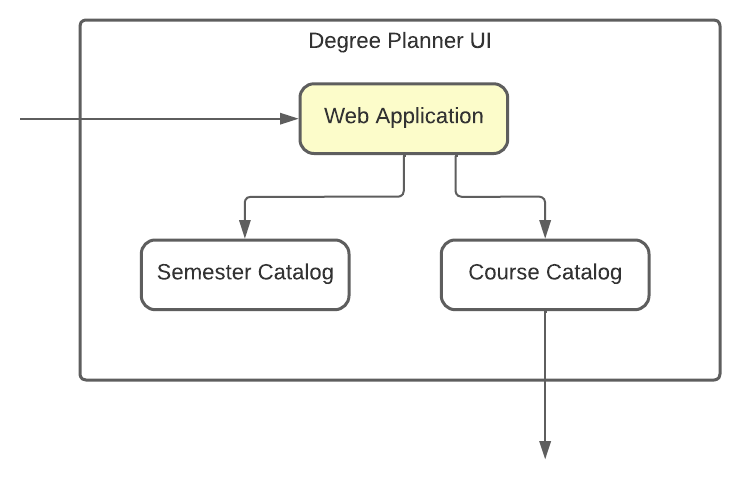
\includegraphics[width=0.60\textwidth]{images/WebApplication}
 \caption{Web Application subsystem}
\end{figure}

\subsubsection{Assumptions}
\begin{itemize}
\begin{item}
The user must have Internet connection to use the service.
\end{item}
\begin{item}
The subsystem is only available for users authenticated in Dashboard layer.
\end{item}
\begin{item}
The subsystem does not provide any functionality to modify data and no data changes should be made in this subsystem.
\end{item}
\end{itemize}

\subsubsection{Responsibilities}
This subsystem takes responsibility to display the required information, including: the user's major, list of courses for the corresponding major, list of semesters, estimated graduation date, total hours per semester, and etc. All data fetched from external sources are assumed to be up-to-date and cannot be modified in this layer. The user will perform planning tasks, such as drag and drop to add and/or remove courses. That is, the list of course objects from Course catalog subsystem will be made draggable, while the area/column for each available semester will become droppable. Besides, there will be navigation options to link to Export subsystem.

\subsubsection{Subsystem Interfaces}

\begin {table}[H]
\caption {Web Application subsystem interfaces} 
\begin{center}
    \begin{tabular}{ | p{1cm} | p{2cm} | p{6cm} | p{3cm} |}
    \hline
    ID & Description & Inputs & Outputs \\ \hline
    \#1 & Choose major & \pbox{6cm}{Option} & \pbox{3cm}{Screen}  \\ \hline
    \#2 & Display courses & \pbox{6cm}{Object of every element in the list of courses provided by Course catalog subsystem} & \pbox{3cm}{Screen}  \\ \hline
    \#3 & Search for courses & \pbox{6cm}{Text \\ Numbers} & \pbox{3cm}{Object of the searched course}  \\ \hline
    \#4 & Display semesters & \pbox{6cm}{List of semesters} & \pbox{3cm}{Screen}  \\ \hline
    \#5 & Export & \pbox{6cm}{N/A} & \pbox{3cm}{Navigation to Export subsystem}  \\ \hline
    \end{tabular}
\end{center}
\end{table}

\subsection{Course Catalog}
Course catalog subsystem acts as the interface between the Degree Planner UI layer and Firebase database layer. It will fetch data, i.e., the list of courses, from the database, and sends it to the Web application subsystem.

\begin{figure}[h!]
	\centering
 	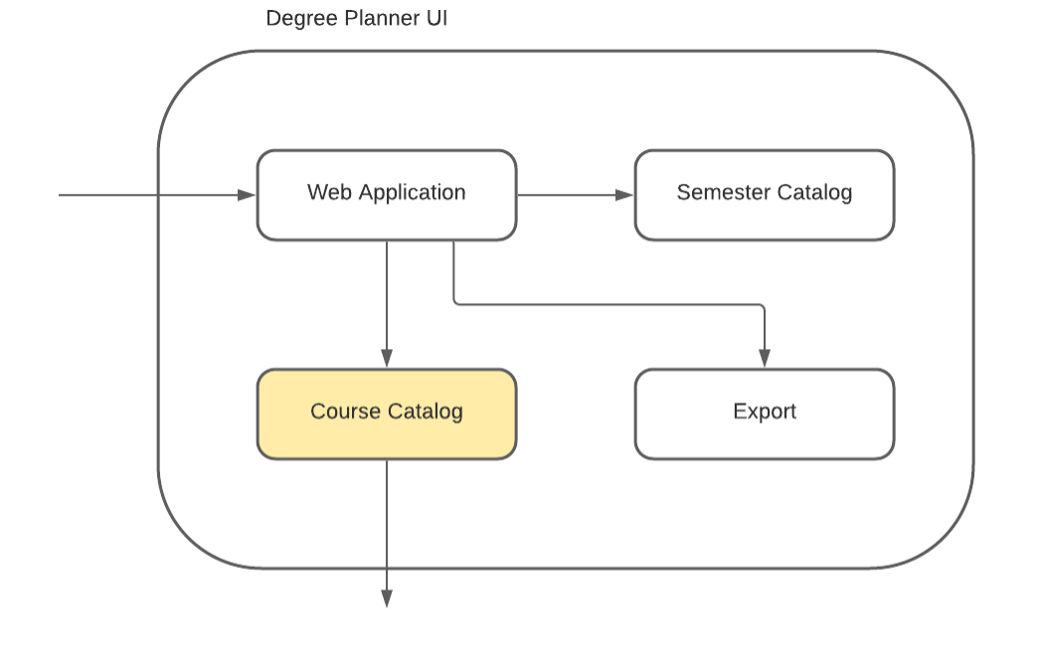
\includegraphics[width=0.60\textwidth]{images/CourseCatalog}
 \caption{Course Catalog subsystem}
\end{figure}

\subsubsection{Assumptions}
\begin{itemize}
\begin{item}
The user must have Internet connection.
\end{item}
\begin{item}
The subsystem gets the raw data from the Firebase layer.
\end{item}
\begin{item}
The subsystem fetches the up-to-date required data from the Firebase layer.
\end{item}
\begin{item}
The subsystem cannot modify data fetched from the Firebase database. It does not provide any functionality to modify data and no data changes should be made in this subsystem.
\end{item}
\end{itemize}

\subsubsection{Responsibilities}
This subsystem will take input, i.e., major, from the web application subsystem, and fetch the corresponding list of courses. Since the database only provides raw data, this subsystem will process each query to create a course object. The list of course objects will then pass to the Web application subsystem.

\subsubsection{Subsystem Interfaces}

\begin {table}[H]
\caption {Course Catalog subsystem interfaces} 
\begin{center}
    \begin{tabular}{ | p{1cm} | p{3cm} | p{2cm} | p{7cm} |}
    \hline
    ID & Description & Inputs & Outputs \\ \hline
    \#1 & Fetch data & \pbox{3cm}{Text} & \pbox{7cm}{Database response with the list of courses from selected major}  \\ \hline
    \#2 & Process data & \pbox{3cm}{Queries} & \pbox{7cm}{List of objects}  \\ \hline
    \end{tabular}
\end{center}
\end{table}

\subsection{Semester Catalog}
Semester catalog subsystem acts as the interface between the Degree Planner UI layer and Dashboard layer. It will read data, i.e., the starting semester, from the user information, and sends it to the Web application subsystem.

\begin{figure}[h!]
	\centering
 	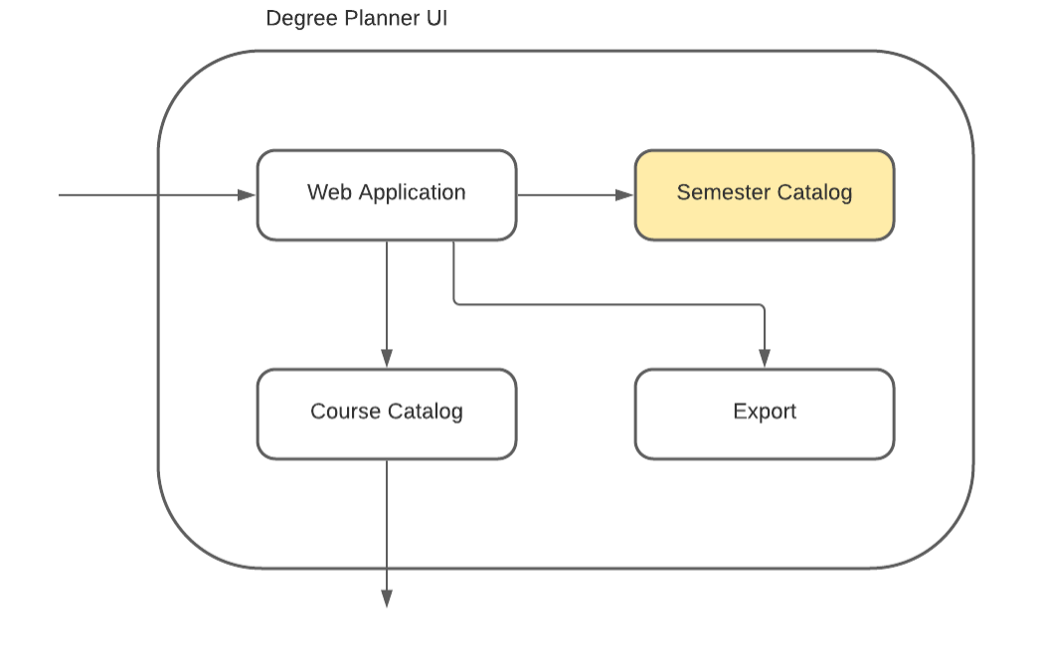
\includegraphics[width=0.60\textwidth]{images/SemesterCatalog}
 \caption{Semester Catalog subsystem}
\end{figure}

\subsubsection{Assumptions}
\begin{itemize}
\begin{item}
The user must have Internet connection.
\end{item}
\begin{item}
The subsystem cannot modify data fetched from the Dashboard. It does not provide any functionality to modify data and no data changes should be made in this subsystem.
\end{item}
\end{itemize}

\subsubsection{Responsibilities}
This subsystem automatically reads the user's starting semester and returns the list of all valid and available semesters to the Web application subsystem. That is, the estimated duration for pursuing a degree in the department of Computer Science and Engineering at the University of Texas at Arlington is 4 years; therefore, the maximum duration for degree completion would be 10 years. The list of semesters will include the starting semester and all subsequent semesters in the next 10 years.

\subsubsection{Subsystem Interfaces}

\begin {table}[H]
\caption {Semester Catalog subsystem interfaces} 
\begin{center}
    \begin{tabular}{ | p{1cm} | p{3cm} | p{2cm} | p{7cm} |}
    \hline
    ID & Description & Inputs & Outputs \\ \hline
    \#1 & Fetch data & \pbox{2cm}{N/A} & \pbox{7cm}{List of semesters in the next 10 years from the staring semester}  \\ \hline
    \end{tabular}
\end{center}
\end{table}


\newpage
\section{Firebase Layer}
% In this section, the layer is described in terms of the hardware and software design. Specific implementation details, such as hardware components, programming languages, software dependencies, operating systems, etc. should be discussed. Any unnecessary items can be omitted (for example, a pure software module without any specific hardware should not include a hardware subsection). The organization, titles, and content of the sections below can be modified as necessary for the project.
The Degree Planner Firebase Layer consists of two subsystems, Authentication and Firestore Database. It is reposible for authenticating the user and retrieving their information. The database function will return null unless the user has been authenticated with Firebase.

\subsection{Layer Hardware}
% A description of any involved hardware components for the layer. For example, if each subsystem is a software process running on an embedded computer, discuss the specifics of that device here. Do not list a hardware component that only exists at the subsystem level (include it in the following sections).
The Firebase layer is dependent on Firebase servers hosted by Google.

\subsection{Layer Operating System}
% A description of any operating systems required by the layer.
Google's Firebase does not publish what operating system their servers run on.

\subsection{Layer Software Dependencies}
% A description of any software dependencies (libraries, frameworks, etc) required by the layer.
The Firebase layer uses JavaScript/TypeScript to make requests to Firebase. It is dependent on the firebase-core package. This package is required for both subsystem's software dependencies.

\subsection{Authentication Subsystem}
Describe at a high level the purpose and basic design of this subsystem. Is it a piece of hardware, a class, a web service, or something else? Note that each of the subsystem items below are meant to be specific to that subsystem and not a repeat of anything discussed above for the overall layer.

%%%%%%%%%%%%%%%%%%%%%%%%%%%%%%%%%%%%%%%%%%%%%%%%%%%%%%%%%%
%  BE SURE TO UPDATE THE IMAGE CAPTION
\begin{figure}[h!]
	\centering
	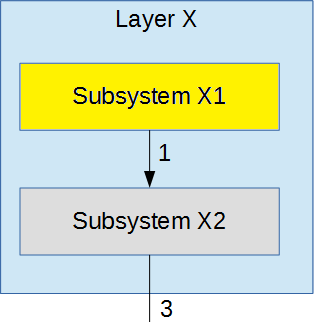
\includegraphics[width=0.60\textwidth]{images/subsystem} % Image
	\caption{Example authentication subsystem description diagram} % Caption
\end{figure}

% \subsubsection{Subsystem Hardware}
% A description of any involved hardware components for the subsystem.

% \subsubsection{Subsystem Operating System}
% A description of any operating systems required by the subsystem.

\subsubsection{Subsystem Software Dependencies}
% A description of any software dependencies (libraries, frameworks, design software for mechanical parts or circuits, etc) required by the subsystem.
The Authentication Subsystem is dependent on the firebase-auth package to authenticate the user before they can use the website.

\subsubsection{Subsystem Programming Languages}
% A description of any programming languages used by the subsystem.
The Authentication Subsystem is programmed using TypeScript.

\subsubsection{Subsystem Data Structures}
% A description of any classes or other data structures that are worth discussing for the subsystem. For example, data being transmitted from a microcontroller to a PC via USB should be first be assembled into packets. What is the structure of the packets?
The Authentication Subsystem has all authentication functions in one file, and each function is exported. This allows for the server to take advantage of tree shaking, which means only code needed is imported and not the entire file.

% \subsubsection{Subsystem Data Processing}
% A description of any algorithms or processing strategies that are worth discussing for the subsystem. If you are implementing a well-known algorithm, list it. If it is something unique to this project, discuss it in greater detail.

\subsection{Firestore Database Subsystem}
% Describe at a high level the purpose and basic design of this subsystem. Is it a piece of hardware, a class, a web service, or something else? Note that each of the subsystem items below are meant to be specific to that subsystem and not a repeat of anything discussed above for the overall layer.
The Firestore Database Subsystem is responsible for retrieving user information, their chosen courses, and a list of all courses from the Firebase Firestore Database.

%%%%%%%%%%%%%%%%%%%%%%%%%%%%%%%%%%%%%%%%%%%%%%%%%%%%%%%%%%
%  BE SURE TO UPDATE THE IMAGE CAPTION
\begin{figure}[h!]
	\centering
	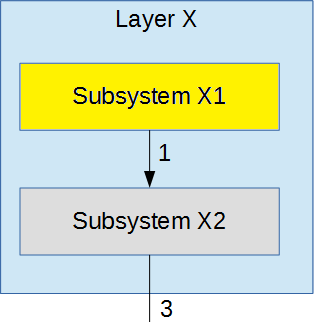
\includegraphics[width=0.60\textwidth]{images/subsystem} % Image
	\caption{Example database subsystem description diagram} % Caption
\end{figure}

% \subsubsection{Subsystem Hardware}
% A description of any involved hardware components for the subsystem.

% \subsubsection{Subsystem Operating System}
% A description of any operating systems required by the subsystem.

\subsubsection{Subsystem Software Dependencies}
% A description of any software dependencies (libraries, frameworks, design software for mechanical parts or circuits, etc) required by the subsystem.
The Firestore Database Subsystem is dependent on the firebase-firestore package to make database queries to the Firestore Database.

% \subsubsection{Subsystem Programming Languages}
% A description of any programming languages used by the subsystem.

\subsubsection{Subsystem Data Structures}
% A description of any classes or other data structures that are worth discussing for the subsystem. For example, data being transmitted from a microcontroller to a PC via USB should be first be assembled into packets. What is the structure of the packets?
The Firebase Database Subsystem has all authentication functions in one file, and each function is exported. This allows for the server to take advantage of tree shaking, which means only code needed is imported and not the entire file.

\subsubsection{Subsystem Data Processing}
% A description of any algorithms or processing strategies that are worth discussing for the subsystem. If you are implementing a well-known algorithm, list it. If it is something unique to this project, discuss it in greater detail.
The Firebase Database Subsystem processes the data received from Firestore and converts it to Class Objects to take advantage of static analysis.

The subsystem converts the JSON string received from the all courses list in Firestore and converts it to a list of Courses objects.

The subsystem converts the user information stored in Firestore and converts it to the object UserData. When processing the user information, it also converts the user's chosen classes to the ChosenCourse object. The ChosenCourse object is a minified version of Course with an id reference to the Course object with the full details.

\newpage
\section{Dashboard Layer}
In this section, the layer is described in some detail in terms of its specific subsystems. Describe each of the layers and its subsystems in a separate chapter/major subsection of this document. The content of each subsystem description should be similar. Include in this section any special considerations and/or trade-offs considered for the approach you have chosen.

\subsection{Subsystem 1}
This section should be a general description of a particular subsystem for the given layer. For most subsystems, an extract of the architectural block diagram with data flows is useful. This should consist of the subsystem being described and those subsystems with which it communicates.

\begin{figure}[h!]
	\centering
 	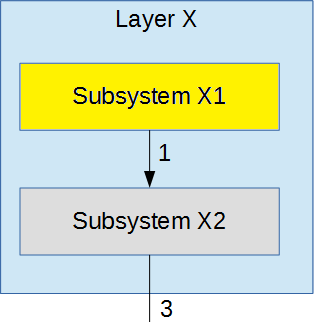
\includegraphics[width=0.60\textwidth]{images/subsystem}
 \caption{Example subsystem description diagram}
\end{figure}

\subsubsection{Assumptions}
Any assumptions made in the definition of the subsystem should be listed and described. Pay particular attention to assumptions concerning interfaces and interactions with other layers.

\subsubsection{Responsibilities}
Each of the responsibilities/features/functions/services of the subsystem as identified in the architectural summary must be expanded to more detailed responsibilities. These responsibilities form the basis for the identification of the finer-grained responsibilities of the layer's internal subsystems. Clearly describe what each subsystem does.

\subsubsection{Subsystem Interfaces}
Each of the inputs and outputs for the subsystem are defined here. Create a table with an entry for each labelled interface that connects to this subsystem. For each entry, describe any incoming and outgoing data elements will pass through this interface.

\begin {table}[H]
\caption {Subsystem interfaces} 
\begin{center}
    \begin{tabular}{ | p{1cm} | p{6cm} | p{3cm} | p{3cm} |}
    \hline
    ID & Description & Inputs & Outputs \\ \hline
    \#xx & Description of the interface/bus & \pbox{3cm}{input 1 \\ input 2} & \pbox{3cm}{output 1}  \\ \hline
    \#xx & Description of the interface/bus & \pbox{3cm}{N/A} & \pbox{3cm}{output 1}  \\ \hline
    \end{tabular}
\end{center}
\end{table}

\subsection{Subsystem 2}
Repeat for each subsystem

\subsection{Subsystem 3}
Repeat for each subsystem


\newpage

%%% References
\bibliographystyle{plain}
\bibliographystyle{reference/IEEEtran_custom}
\bibliography{reference/refs}{}

\end{document}